\documentclass{scrreprt}
\usepackage{scrhack}
\KOMAoptions
{
  draft,
  DIV=calc, % this will calculate correct margins
  fontsize=12pt,
  listof=numbered,
}

\usepackage[english]{babel}

\usepackage[autostyle]{csquotes}

\usepackage[backend=biber,style=alphabetic]{biblatex}
\addbibresource{Bibliography.bib}

% Alternative to `Helvetica': TeX Gyre Heros
% Alternative to `Bookman Old Style': TeX Gyre Bonum
\usepackage{fontspec}
\setromanfont{TeX Gyre Bonum} % Enhanced version of `Bookman Old Style'.
\setmonofont{Consolas}
% \setsansfont{TeX Gyre Heros} % Replacement for Helvetica.

% Choose default font family.
%
% Options:
%   \rmdefault   Use the serif font family as default.
%   \sfdefault   Use the sans-serif font family as default.
%   \ttdefault   Use the monospace font family as default.
\renewcommand{\familydefault}{\sfdefault}

\usepackage{ifdraft}
\usepackage{amsmath}

\PassOptionsToPackage{draft}{graphicx}
\usepackage{graphicx}

\usepackage[toc,page]{appendix}

\usepackage{todonotes}

\usepackage[acronym]{glossaries}
%!TEX root = ../Main.tex


%
% Acronyms
%

\newacronym{api}{API}{Application Programming Interface}
\newacronym{cpu}{CPU}{Central Processing Unit}
\newacronym{gpu}{GPU}{Graphics Processing Unit}
\newacronym{ram}{RAM}{Random Access Memory}
\newacronym{vram}{VRAM}{Video Random Access Memory}
\newacronym{gui}{GUI}{Graphical User Interface}
\newacronym{2d}{2D}{two-dimensional}
\newacronym{3d}{3D}{three-dimensional}

\newacronym{glsl}{GLSL}{OpenGL Shading Language}
\newacronym{spir}{SPIR}{Standard Portable Intermediate Representation}
\newacronym{spirv}{SPIR-V}{Standard Portable Intermediate Representation version `V'}

\newacronym{ps3}{PS3}{Sony PlayStation 3}
\newacronym{ps4}{PS4}{Sony PlayStation 4}
\newacronym{xbox360}{Xbox 360}{Xbox 360}
\newacronym{xbone}{Xbox One}{Xbox One}


%
% Glossary Entries
%

\newglossaryentry{host}
{
  name={host},
  description={The user of the Vulkan API}
}
\newglossaryentry{device}
{
  name={device},
  description={The GPU abstracted by the Vulkan API}
}
\newglossaryentry{application}
{
  name={application},
  description={The user of or the developer that uses the Vulkan API}
}
\newglossaryentry{driver}
{
  name={Vulkan implementation},
  description={The part of the Vulkan API that is opaque to the user, implemented in the hardware driver}
}


\usepackage{xcolor}
\definecolor{CodeComment}{gray}{0.4}
\definecolor{CodeKeyword}{rgb}{0.0,0.0,0.8}
\definecolor{CodeString}{rgb}{0.0,0.3,0.0}

\usepackage{listings}
\lstdefinestyle{MyCpp}
{
  language=[11]C++,
  % backgroundcolor=\color{backcolour},
  commentstyle=\color{CodeComment},
  keywordstyle=\color{CodeKeyword},
  numberstyle=\ttfamily\color{CodeComment},
  stringstyle=\color{CodeString},
  basicstyle=\ttfamily,
  breakatwhitespace=false,
  breaklines=true,
  captionpos=b,
  keepspaces=true,
  numbers=left,
  numbersep=5pt,
  showspaces=false,
  showstringspaces=false,
  showtabs=false,
  tabsize=2
}
\lstset{style=MyCpp}

\usepackage{hyperref}
\hypersetup{
  colorlinks,
  final,
  bookmarksnumbered,
  citecolor=black,
  filecolor=black,
  linkcolor=black,
  urlcolor=black
}

\usepackage[nopar]{lipsum}
\setlipsumdefault{1}


\title{Evaluating the Resource Management Possibilites of the Vulkan Graphics API
  \todo[inline, color=red!64]{\centerline{DRAFT}}
}

\date{\today}
\author{Manuel Maier}

\begin{document}
  %
  % Title Page
  %
  \pagenumbering{gobble}
  \maketitle


  %
  % Blank page for physical notes, name entries, etc.
  %
  \newpage
  \null
  \pagenumbering{gobble}

  %
  % Abstract and acknoledgements.
  %
  %!TEX root = ../Main.tex

\chapter*{Abstract}
\label{cha:Abstract}

This is the abstract.

\lipsum[1-2]

  %!TEX root = ../Main.tex

\chapter*{Acknowledgements}
\label{cha:Acknowledgements}

These are my acknowledgements.

\todo[inline]{Make proper sentences below.}

\paragraph{Stefan Radicke}
  supervision.
  Lorem ipsum dolor sit amet, consectetuer adipiscing elit. Aenean commodo ligula eget dolor. Aenean massa. Cum sociis natoque penatibus et.

\paragraph{Patrick Bader}
  supervision.
  Lorem ipsum dolor sit amet, consectetuer adipiscing elit. Aenean commodo ligula eget dolor. Aenean massa. Cum sociis natoque penatibus et.

\paragraph{Hannes Pernpeinter}
  discussion, proof-reading.
  Lorem ipsum dolor sit amet, consectetuer adipiscing elit. Aenean commodo ligula eget dolor. Aenean massa. Cum sociis natoque penatibus et.

\paragraph{Christopher Manthei}
  discussion, proof-reading, experience.
  Lorem ipsum dolor sit amet, consectetuer adipiscing elit. Aenean commodo ligula eget dolor. Aenean massa. Cum sociis natoque penatibus et.

\paragraph{Benjamin Thaut}
  ???.
  Lorem ipsum dolor sit amet, consectetuer adipiscing elit. Aenean commodo ligula eget dolor. Aenean massa. Cum sociis natoque penatibus et.

\paragraph{Maria Floruß}
  rubber-ducking, proof-reading, support.
  Lorem ipsum dolor sit amet, consectetuer adipiscing elit. Aenean commodo ligula eget dolor. Aenean massa. Cum sociis natoque penatibus et.



  %
  % Table of Contents
  %
  \newpage
  \pagenumbering{roman}
  \tableofcontents
  \newpage


  %
  % Chapters
  %
  \pagenumbering{arabic}
  %!TEX root = ../Main.tex

\chapter{Introduction}
\label{cha:Introduction}
  \todo[inline]
  {
    Brief introduction of computer graphics. One of the biggest problems: Performance. Especially on mobile and with virtual reality.

    Maybe mention the author's (that's me!) bias towards game development.

    Mention target audience requirements?

    Explain shader stages of modern graphics hardware somewhere in this chapter.
  }

  \todo[inline]{Mention the terms \gls{cpu} and \gls{gpu} here somewhere.}

  % The field of computer graphics poses many challenges.

  % Data is consumed by a pipeline and transformed by complex algorithms, resulting in another set of data that is used in further processing. This transformation process is usually referred to as ``rendering''. In its most simple form, the output of the rendering process is used to present a graphical representation of the input data to the user, typically via a computer monitor peripheral device.

  % Computer graphics is an area of computer science that has many disciplines. Examples are \glspl{gui}, computer vision, sprite graphics, and \gls{3d} modelling. Most relevant to this paper is \gls{3d} computer graphics. \todo{Mention how Vulkan is not only suited for \gls{3d} graphics?} The most typical use case in \gls{3d} computer graphics is to process data, usually three-dimensional geometric data, in order to produce a 2D image which is then presented to the user with the help of a computer monitor. This processing of data is referred to as \textit{3D rendering} or simply \textit{rendering}.

  % While 3D rendering can be implemented in software, special hardware called a \gls{gpu} can be used instead to achieve better performance. The need for such hardware already indicates one of the greatest challenges in 3D computer graphics: performance. The amount of data involved in 3D rendering can become quite large. As an example, assume the following:

  % \todo{Explain what a Vertex is and how graphics hardware produces faces etc.}

  % The aforementioned three-dimensional geometric data can be given in many different ways. The ideal way of representing specific data depends on the use case and the entire 3D graphics pipeline.

  % For the sake of illustration, let's assume a data set that consists only of 3D vertices. In this example, each vertex only has a position defining the absolute location of the vertex in 3D space. This position value is stored as a vector of three floating point numbers. Typically, such floating point numbers are standard IEEE floating point numbers (as per IEEE 754), taking up 32 bits or 4 bytes of memory. Thus, each vertex takes up $3*4 = 12$ bytes of memory.

  % On desktop systems, applications typically don't access the graphics hardware directly. They instead communicate with a driver that manages hardware access. Communication between an applicatin and the driver is done via an \gls{api}. Figure \ref{fig:AppApiDriverOverview} visualizes this relationship. Ideally, the application does not need to know which specific driver it is communicating with as long as the driver is compliant to the \gls{api} specification. This abstraction decouples the application from the hardware and enables it to run on systems with different hardware configurations without altering the application itself. It also enables hardware vendors to manipulate or even reject operations requested by the application, typically to enforce some user-specified global settings. \todo{Explain what kind of settings? Maybe give an example?}

  \begin{figure}
    \centering
    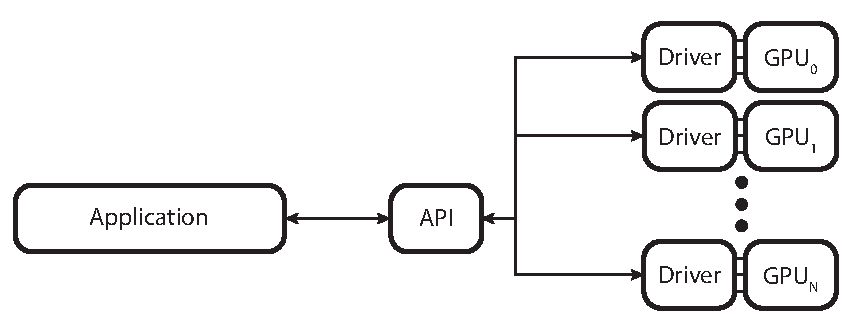
\includegraphics[width=\textwidth]{Main/Images/Application_API_Driver_Overview}
    \caption{Interaction between the application and the hardware via the API.}
    \label{fig:AppApiDriverOverview}
  \end{figure}

  Lorem ipsum dolor sit amet, consectetur adipisicing elit, sed do eiusmod
  tempor incididunt ut labore et dolore magna aliqua. Ut enim ad minim veniam,
  quis nostrud exercitation ullamco laboris nisi ut aliquip ex ea commodo
  consequat. Duis aute irure dolor in reprehenderit in voluptate velit esse
  cillum dolore eu fugiat nulla pariatur. Excepteur sint occaecat cupidatat non
  proident, sunt in culpa qui officia deserunt mollit anim id est laborum.

  Lorem ipsum dolor sit amet, consectetur adipisicing elit, sed do eiusmod
  tempor incididunt ut labore et dolore magna aliqua. Ut enim ad minim veniam,
  quis nostrud exercitation ullamco laboris nisi ut aliquip ex ea commodo
  consequat. Duis aute irure dolor in reprehenderit in voluptate velit esse
  cillum dolore eu fugiat nulla pariatur. Excepteur sint occaecat cupidatat non
  proident, sunt in culpa qui officia deserunt mollit anim id est laborum.

  \todo[inline]{Talk about different kinds of graphics \glspl{api} on different systems (D3D, OpenGL on desktop, maybe Metal for OSX, and special \glspl{api} on consoles.)}

  \section{Document Structure}
    Chapter~\ref{cha:Introduction} is the introduction to the topics discussed within this document.
    In chapter~\ref{cha:VulkanOverview}, an overview of the Vulkan graphics \gls{api} is given in terms of its components and features.
    Chapter~\ref{cha:EnvSetup} is a guide for setting up Vulkan for application development with a bias towards \gls{windows} platforms.
    Chapter~\ref{cha:RenderPipeline} sets up a simple rendering scenario and explains it step by step.
    And finally, chapter~\ref{cha:Conclusion} concludes this document and provides insight to thoughts of the author about the topics discussed.


  \section{High Level Graphics Workflow}
    \label{sec:GraphicsWorkflow}
    \todo[inline]
    {
      General overview of the stages several resources (vertices, textures, etc.) have to go through.

      Explain the fixed function stages.

      Mention that this is simplified!!! Mention there are more stages.
    }

    \todo[inline]{Change the text ``Vertex Data'' to ``Input Data'' in figure~\ref{fig:Rendering_Pipeline_Overview}.}
    \begin{figure}
      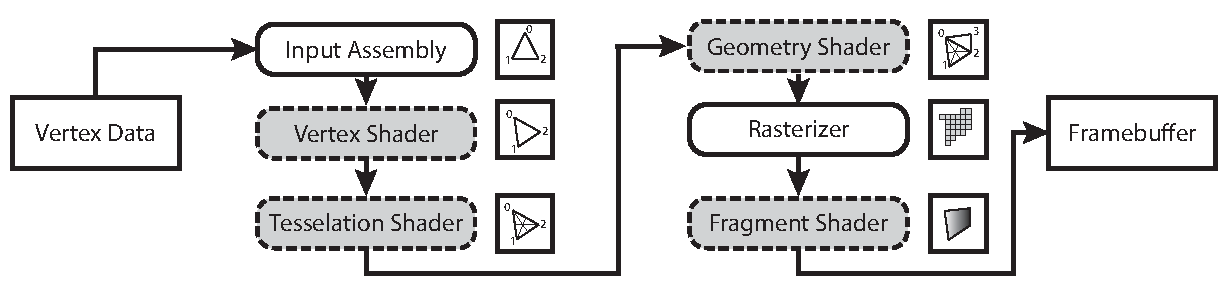
\includegraphics[width=\textwidth]{Main/Images/Rendering_Pipeline_Overview}
      \centering
      \caption{Fixed-function stages are depicted with solid, rounded outlines and shader stages with dashed outlines.}
      \label{fig:Rendering_Pipeline_Overview}
    \end{figure}

    Generally speaking, graphics hardware is built like a pipeline that is made up of several components called pipeline stages.
    Each of these stages is processing data that is provided by the \textit{host application}, before being passed on to the next stage in the pipeline.
    The pipeline stages can generally be categorized into fixed-function stages and shader stages.
    Fixed-function stages perform the same kind of operation on incoming data.
    Control over the operation is limited, but in many cases a fixed-function stage can be configured to some extent.
    Shader stages accept application-defined programs, called \textit{shaders}, that are run in order to process incoming data.
    \todo{...}Overview of the rendering pipeline on modern graphics hardware.
    The available shader stages are the vertex, tessellation, geometry, and fragment shader stages.

    % The input assembly, for example, is responsible for producing primitives from the input data for the vertex shader to consume.

    \begin{description}
      \item[Vertex Shader]
        Vertex shaders are invoked for individual vertices.
        This stage is typically used to transform vertices to different coordinate systems.

      \item[Tessellation Shader]
        Tessellation shaders are generally used to turn coarse geometry into smoother geometry by adding more detail.
        \todo[inline]{Used for water, e.g. or to create a mathematical ...}

      \item[Geometry Shader]
        Geometry shaders are used to generate new geometry from existing primitives.
        For example, the geometry shader may be used to turn a single vertex into a triangle.

      \item[Fragment Shader]
        Fragment shaders work on individual output pixels to determine values that are written to the framebuffer.
        In other words, this is the stage where the actual pixel colors are produced, optionally by sampling textures and applying lighting computations.
    \end{description}

    \todo[inline]{Is this enough for the \underline{high level} graphics workflow?}

  \section{Motivation for a new Graphics API}
    \todo[inline]{Hardware abstraction of old APIs based on old hardware design.
    \todo[inline]{Check for repetition.}
    Hardware design changed a lot (much more general purpose).
    Old APIs need to perform a lot of work to maintain the illusion of old hardware design.
    Special purpose hardware is largely replaced by general purpose memory and massively parallel processors for crunching data.}
    \todo[inline]{Different Formulation. Graphics hardware changes rapidly, etc...}
    Old graphics \glspl{api} were designed for old graphics hardware designs.
    However, hardware design has changed significantly over time.
    The model older graphics \glspl{api} are based on no longer reflects modern hardware design.
    In order to remain compatible, these \glspl{api} need to perform a mapping of their model to modern hardware design.
    This mapping may come at a significant cost in terms of performance.

    In practice, this often means that the hardware driver, implementing an old graphics \gls{api}, wastes a considerable amount of time that could be used by the host application to perform useful \todo{Use `operations' instead?}computations.
    For some applications, this \todo{``may be acceptible...'' is clearer}overhead caused by the driver is not very significant.
    Applications like these may not gain much by the new \glspl{api} other than lower power consumption due to reduced \gls{cpu} usage, which might be important on mobile platforms.

    Modern hardware design tends to be more suitable for general purpose computing compared to old hardware design.
    Older hardware consisted of many special purpose components that have largely been replaced by general purpose memory and programmable processing cores that perform work in a massively parallel manner.

    \todo[inline]{Main goal of modern APIs is to match modern hardware design. Enables drivers to work more directly with the hardware instead of perform a mapping between the abstract model and the actual hardware.}

    Modern graphics \glspl{api} match their abstraction closer to modern hardware design.
    This enables drivers to work more directly with the hardware and reduce the aforementioned cost of mapping the driver model to the actual hardware.
    This is arguably the main motivation for new graphics \glspl{api}.

    Another aspect of modern graphics \glspl{api} is the level of control that is given to the application.
    \todo{Don't be abstract: Mention directX, opengl, i.e. the established apis}Modern \glspl{api} tend to design their model much closer to the current hardware, exposing it a lot more than older \glspl{api} did.
    The fact that modern graphics hardware has become more general purpose is certainly a factor in this.
    Designing general purpose hardware only to be constrained by \glspl{api} that do not provide ways to leverage it would be a waste of resources.
    \todo{References??}Additionally, having more control of the hardware has been the desire of many developers in the past.
    On gaming consoles, for example, working closely with graphics hardware has been always possible\footnote{Except on \gls{ms} platforms where \gls{d3d} technology is used.}.
    A game ported from a console to a platform \todo{``such as''?}like the \gls{pc} would often run less optimal in comparison in terms of the most optimal use of available resources.

    Providing more control to the application also means that drivers have to do less guess-work to figure out what the application wants to do.
    This makes driver implementations simpler and easier to maintain, reducing the possibility for \glspl{bug}.
    \todo{Application developers have a better chance to optimize for different hardware.}
    \todo[inline]{The following sentence is not correct. Reformulate.}
    It also reduces the gap between different driver implementations, making applications work more consistently across hardware from different vendors.

    \todo[inline]{Secondary goal is to make drivers simpler at the cost of making applications more complicated. This is not necessarily bad because the application has control over how hardware is utilized. Drivers don't need to guess user intent as much anymore. Also, less complex driver means better maintainability and fewer bugs.}

    Multithreading is also a concern for modern graphics applications.
    With older graphics \glspl{api} it was usually much harder, if not impossible, to utilize multiple threads in terms of rendering.
    At the time these \glspl{api} were designed, applications were usually running only in a single thread.
    Modern graphics \glspl{api}, on the other hand, have been designed with multi-core processing in mind.

    \todo[inline]{Mention CPU overhead of GPU instructions, especially on mobile.}

    \todo[inline]{Talk about new APIs such as D3D12, Mantle, Metal, and also talk about consoles (no specs) that all adress these problems.}


  \section{The Vulkan Graphics and Compute API}
    \todo[inline]{What does it do. Where does it come from. What are people expecting from it. Cross-platform nature (in comparison maybe to PS4's libGNM made specifically for PS4 hardware).}

    \todo[inline]{Insert missing references.}
    The Vulkan \gls{api} was designed by the Khronos Group in collaboration with many industry representatives, including Valve Corporation, \gls{amd}, and \gls{nvidia}.
    Version 1.0 of the Vulkan specification was released on the 16th February in 2016.
    It was designed to provide low-level control to the developer when interacting with graphics and compute hardware.

    Vulkan was designed with a variety of goals in mind.

    \todo[inline]{Will this stay a list?}
    \begin{itemize}
      \item Cross-platform
      \item Keep driver complexity at a minimum
      \item Less driver-side \gls{cpu} overhead
      \item Allow developers a lot of control over the hardware
      \item Consistent API
    \end{itemize}

    There are many different kinds of hardware configurations today, ranging from high-end gaming systems to mobile platforms such as smartphones.
    Vulkan is designed to be used with all of these systems.
    There will be no special version of Vulkan dedicated to embedded systems as was the case with \gls{gles}.

    As a result of striving for less driver overhead, Vulkan also provides the possibility of reducing \gls{cpu} and \gls{gpu} power consumption.
    The driver implementation will have to make fewer guesses of what the host application is trying to do.
    It is up to the application developer to tell the Vulkan driver exactly what needs to be done.
    This way the driver only does as much work as it needs to function properly and less power will be consumed.
    Hardware vendors will also have an easier time providing robust drivers with less bugs due to reduced complexity.

    Another advantage of Vulkan, being a new API built without worrying about backwards compatability, is the chance of designing a new and consistent API so developers will have an easier time creating applications.
    For more information about the API structure and common patterns in Vulkan, see chapter~\ref{cha:VulkanOverview}.

    Version 1.0 of Vulkan was not entirely built in-house at Khronos Group but is in part based on components of AMD's Mantle API, which was donated to the Khronos Group.


    \subsection{Vulkan Competitors}
      \todo[inline]{OpenGL, Direct3D11, Direct3D12, libGNM (PS4), OpenCL}

      Other \glspl{api} exist that are direct competitors to Vulkan.

      \gls{opengl} is Vulkans predecessor and provides a higher level of abstraction from the hardware.
      It is a very successful API running on several different platforms with varying hardware configurations.
      Due to its level of abstraction, \gls{opengl} drivers are very complex and do a significant amount of work on the \gls{cpu} in order to match abstract commands to the hardware.

      Special flavors of \gls{opengl} exist, such as \gls{gles}, which is a subset of \gls{opengl} to enable hardware-accelerated graphics processing on embedded systems such as smartphones and tablets.

      The \gls{d3d} family of \glspl{api} is developed by Microsoft and only supports Microsoft platforms such as the Windows operating system or the Xbox gaming console.
      The most recent versions of \gls{d3d} are \acrlong{d3d11} and \acrlong{d3d12}.
      \acrlong{d3d11} provides a \todo{Compared to what? Make this un-ambiguous}higher level of abstraction from the hardware, similar to \gls{opengl}.
      It has been around since the release of Windows 7 in 2009.
      \acrlong{d3d12}, the latest revision of the \gls{d3d} specification released in 2015, is comparable to Vulkan in terms of of hardware abstraction.
      It provides much more control to the developer over the hardware.

      \todo[inline]{Mac OS X: Metal}

      \todo[inline]{Gaming console graphics libraries?}

      \todo[inline]{OpenCL as compute API}

  %!TEX root = ../Main.tex

\chapter{Vulkan API Overview/Workflow}
\label{cha:VulkanOverview}
  \todo[inline]
  {
    The Vulkan Graphics \acrfull{api} workflow, object creation, patterns (vkCreate/vkDestroy, vkAllocate/vkDeallocate), synchronization.

    Listing and short explanation of Vulkan components such as buffers, images, command buffers.

    Note that when talking about a ``device'', a logical device is meant. When referring to the actual hardware component the term ``physical device'' will be used.
  }

  \todo[inline]{Object/handle based with state-machines only for command buffers.}

  \lipsum

  \section{Workflow and Patterns}
  \label{sec:WorkflowAndPatterns}
    \lipsum

  \section{Layers and Extensions}
    \todo[inline]{Layers are instance-only, extensions are both on the isntance-level as well as the device-level.}

    Vulkan is designed to be extensible by thirdparty developers. The two mechanisms provided are called layers and extensions.

    A layer in Vulkan can be thought of as an observer to the API calls done by the developer. It does not add new types or functions the developer can use directly.\todo{Illustration of Vulkan with some layers between it and the user}\todo{Elaborate more to make it crystal clear. Make sure to mention no layers are needed.}

    The LunarG SDK, for example, comes with a set of layers to validate usage of the Vulkan API. This is extremely useful during development as it allows the developer to focus on their code rather than the perfect use of the Vulkan API. It should also be noted that bare Vulkan, without any validation layers enabled, does not do any error checking. When the developer passes an invalid combination of flags to some Vulkan function, it is undefined behavior and has to be corrected by the developer.

    Layers can only be created on the instance-level. Until version x.x.x.x \todo{Find out the exact version.}, the developer was able to create device-level layers, but these are deprecated in Vulkan version x.x.xx.x by now.

    \todo[inline]{Pull out neutral descriptions of layers/extensions and put the examples in their own paragraph.}

    As opposed to layers, extensions are able to provide new or add to existing functionality. The motivation for extensions is to keep the Vulkan core functionality small and provide specific functionality via such extensions. In fact, the Khronos Group itself provides built-in extensions for both common and platform specific functionality. An example of an extension that adds platform independent functionality is the \lstinline{VK_KHR_swapchain} extension. It adds several types and functions to create and interact with a swapchain. The concept of a swapchain itself is independent of the platform but it requires the help of platform specific functionality in order to work. On Windows platforms, for example, the developer needs to enable the \lstinline{VK_KHR_win32_surface} extension in order link a swapchain to a Win32 window. From a developer's perspective, they do not have to care about distinguish between platforms when creating a swapchain but they do have to when creating and connecting the swapchain to a surface.

    Extensions can be enabled on both instance-level and device-level. Instance-level extensions provide functionality that is generally independent of the hardware.

    An example for an instance-level extension is \lstinline{VK_EXT_debug_report}. It enables the developer to provide a callback function that is used by Vulkan layers or extensions to communicate with the developer. If validation layers are enabled, this is how they would tell the developer about any validation concerns or violations. An example for a device-level extension is the aforementioned \lstinline{VK_KHR_swapchain} extension. Not all physical devices have to be capable of rendering graphics images. In the end it is up the extension author on which level they provide their extension.

  \section{Memory Management}
    \todo[inline]{Allocate memory separately and then binding it to resources. Decoupled on purpose for custom management.}

    Memory management is an important topic in Vulkan.

    \lipsum

  \section{Shader Language: SPIR-V}
    \todo[inline]{\acrfull{spirv}}

    \lipsum

  \section{Synchronisation Primitives}
    \todo[inline]{Describe what Vulkan offers and discuss the individual use-cases as well as their performance impact.}

    \lipsum

  \section{Interaction with the Operating System}
    \todo[inline]{Windowing system, specific Vulkan extensions per OS.}

    \lipsum

  %!TEX root = ../Main.tex

\chapter{Vulkan GPU Resources}
\label{cha:GpuResources}
  \todo[inline]
  {
    Different kinds of resources for different kinds of operations. These have been introduced in the previous chapter already and will now be explained in more detail.
  }

  \todo[inline]
  {
    Possible pattern per section: What is the resource used for $\rightarrow$ How is it allocated $\rightarrow$ Discuss synchronisation issues.
  }

  \tbd

  \section{Images and Buffers}
    \todo[inline]{Difference and why it matters.}

    \tbd

  \section{Command Buffers}
    \todo[inline]{Record commands into buffers that are uploaded to the gpu to be replayed there.}

    \tbd

  \section{Shaders and Pipelines}
    \todo[inline]
    {
      Data flow between CPU and GPU. Data flow within the GPU through shaders.

      Descriptor pool/layout/set/set-layout
    }

    \tbd

  %!TEX root = ../Main.tex

\chapter{Resource Management Techniques}
\label{cha:ResourceManagementTechniques}
  \todo[inline]{Discuss what to do in certain situations, e.g. when uploading image data using a staging buffer.}

  \lipsum

  %!TEX root = ../Main.tex

\chapter{Evaluation}
\label{cha:Evaluation}
  \todo[inline]{Present and discuss preformance measurement results.}

  \tbd

  %!TEX root = ../Main.tex

\chapter{Conclusion}
\label{cha:Conclusion}
  \todo[inline]
  {
    API quality. Explain and discuss why the API is called `modern', `highly efficient', and `explicit'.
  }

  \tbd



  \newpage
  \pagenumbering{Roman}


  %
  % Bibliography
  %
  \newpage
  \printbibliography[heading=bibintoc,title=Bibliography]
  \nocite{*} % Make sure to print all bibliography entries.

  %
  % Appendix
  %
  %!TEX root = ../Main.tex

\appendix

%
% List of Figures
%
% \chapter{List of Figures}
% \label{cha:ListOfFigures}
% \cleardoublepage
% \phantomsection
% \addcontentsline{toc}{section}{\listfigurename}
% \begingroup
%   \let\clearpage\relax
%   \listoffigures
% \endgroup
\listoffigures

%
% List of Tables
%
% \chapter{List of Tables}
% \label{cha:ListOfTables}
% \cleardoublepage
% \phantomsection
% \addcontentsline{toc}{section}{\listtablename}
% \begingroup
%   \let\clearpage\relax
%   \listoftables
% \endgroup
\listoftables


\end{document}
